\section{Applying HDM on Testnet}
\nblink{brats/22a\_testnet\_hdm\_circles\_fixed.ipynb}

This chapter shows the Hausdorff Distance Masks method applied on three examples of the testnet.

\subsection{Results}
\begin{figure}[H]
    \centering
    \begin{subfigure}[t]{.28\textwidth}
        \centering
        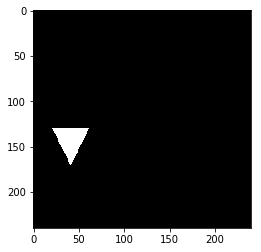
\includegraphics[width=\linewidth]{chapters/06_hdm/testnet/0.png}
        \caption{Ground truth segment}
    \end{subfigure}\hfill%
    \begin{subfigure}[t]{.34\textwidth}
        \centering
        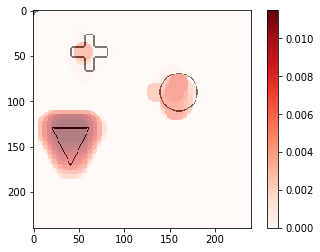
\includegraphics[width=\linewidth]{chapters/06_hdm/testnet/2.png}
        \caption{Regions where the applied masks reduce the accuracy of the segmentation}
    \end{subfigure}\hfill%
    \begin{subfigure}[t]{.36\textwidth}
        \centering
        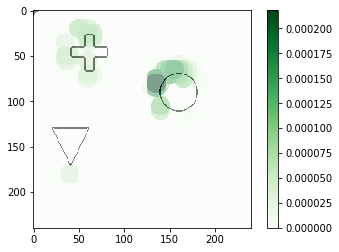
\includegraphics[width=\linewidth]{chapters/06_hdm/testnet/3.png}
        \caption{Regions where the applied masks increase the accuracy of the segmentation}
    \end{subfigure}
    \caption{Visualization (b) and visualization (c) show that both the segmentation region itself and the circle are important for the correct segmentation.}
    \label{hdm_testnet_1}
\end{figure}

\begin{figure}[H]
    \centering
    \begin{subfigure}[t]{.28\textwidth}
        \centering
        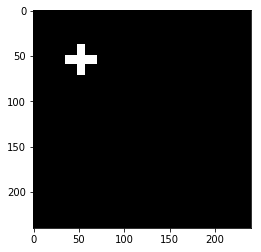
\includegraphics[width=\linewidth]{chapters/06_hdm/testnet/4.png}
        \caption{Ground truth segment}
    \end{subfigure}\hfill%
    \begin{subfigure}[t]{.34\textwidth}
        \centering
        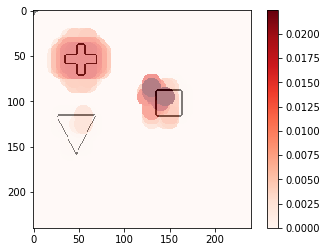
\includegraphics[width=\linewidth]{chapters/06_hdm/testnet/6.png}
        \caption{Regions where the applied masks reduce the accuracy of the segmentation}
    \end{subfigure}\hfill%
    \begin{subfigure}[t]{.34\textwidth}
        \centering
        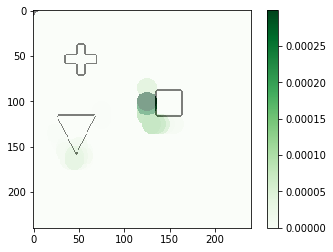
\includegraphics[width=\linewidth]{chapters/06_hdm/testnet/7.png}
        \caption{Regions where the applied masks increase the accuracy of the segmentation}
    \end{subfigure}
    \caption{Similar to above, both the visualization (b) and visualization (c) show that both the segmentation region itself and the square are important for the correct segmentation.}
    \label{hdm_testnet_2}
\end{figure}

\begin{figure}[H]
    \centering
    \begin{subfigure}[t]{.28\textwidth}
        \centering
        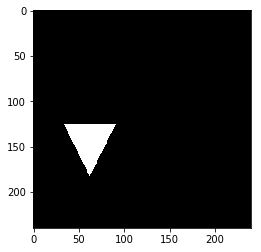
\includegraphics[width=\linewidth]{chapters/06_hdm/testnet/8.png}
        \caption{Ground truth segment}
    \end{subfigure}\hfill%
    \begin{subfigure}[t]{.34\textwidth}
        \centering
        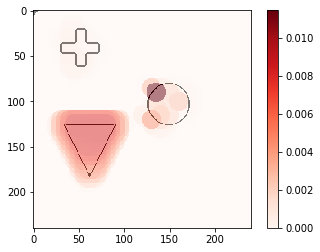
\includegraphics[width=\linewidth]{chapters/06_hdm/testnet/10.png}
        \caption{Regions where the applied masks reduce the accuracy of the segmentation}
    \end{subfigure}\hfill%
    \begin{subfigure}[t]{.34\textwidth}
        \centering
        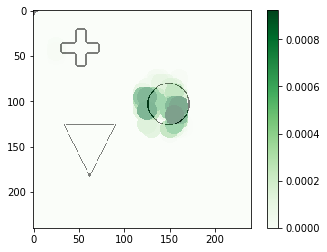
\includegraphics[width=\linewidth]{chapters/06_hdm/testnet/11.png}
        \caption{Regions where the applied masks increase the accuracy of the segmentation}
    \end{subfigure}
    \caption{In this sample, the output looks similar to the two figures above, with slightly different positions for the masks}
    \label{hdm_testnet_3}
\end{figure}

\subsection{Discussion}
All three figures (Figure \ref{hdm_testnet_1}, Figure \ref{hdm_testnet_2} and Figure \ref{hdm_testnet_3}) show the importance of not only the segmented region itself (cross/triangle symbol), but also the symbol on the right which decides which symbol on the left should be segmented. With this dataset, increasing the accuracy (the green visualizations in the figures) by masking parts of the image happens, but the decrease of the Hausdorff distance to the ground truth is quite small in comparison to the distance when the accuracy goes down (red visualizations).

As expected from this dataset, the edges and corners of the right symbols are very important to generate the correct output segment.

\subsection{Conclusion}
The new Hausdorff Distance Masks method shows much better results than the modified RISE method. The importance of the right symbol is clearly visible, even the importance of the edges and corners of the symbols are visible.

After validating the basic functionality of this method, we apply it on the BraTS dataset to see if it also provides useful insight into the neural network model.
